\documentclass[11pt,a4j,uplatex]{jsarticle}
\usepackage{ascmac}
\usepackage{amsmath}
\usepackage[dvipdfmx]{graphicx}
\usepackage{upgreek}
\usepackage{ulem}
\usepackage{bm}%ベクトル表記\bm{なにか}
\usepackage{cases}%連立方程式.

\newsavebox{\circlebox}
\savebox{\circlebox}{\fontencoding{OMS}\selectfont\Large\char13}
\newlength{\circleboxwdht}
\newcommand{\centercircle}[1]{%
  \setlength{\circleboxwdht}{\wd\circlebox}%
  \addtolength{\circleboxwdht}{\dp\circlebox}%
  \raisebox{0.4\dp\circlebox}{%
    \parbox[][\circleboxwdht][c]{\wd\circlebox}{\centering#1}}%
  \llap{\usebox{\circlebox}}%
}	%丸数字(文字)環境。\centercircle{入れたい文字} で丸文字を表示する。


\title{宮島研究室2019年度B4 XRD実験}
\author{東京理科大学 理学部 応用物理学科\\宮島研究室B4 渡辺慧}
\date{\today}


\begin{document}

\maketitle %タイトル

\thispagestyle{empty}%このページにはページ番号を入れない.
\clearpage
\addtocounter{page}{-1}%ページのカウントを-1する.

\newpage

\tableofcontents %目次

\thispagestyle{empty}%このページにはページ番号を入れない
\clearpage
\addtocounter{page}{-1}

%\listoffigures%図目次。確認用。後で消す

\newpage
\section{本研究の目的}
本研究の目的は、X線回折装置によって、Nacl結晶のX線回折パターンを測定し、格子定数の導出を行うことである。

\section{原理}

\subsection{結晶面}

図\ref{a1}(a)のような立方格子を考える。$\bm{a_1}、\bm{a_2}、\bm{a_3}$を各方向への単位ベクトルと考えた時、位置ベクトル$\bm{r}$は$\bm{r}=h\bm{a_1}+k\bm{a_2}+l\bm{a_3}$と表せる。$h,k,l$はミラー指数と呼ばれる。このとき、$\bm{r}$の方向を[$h,k,l$]と表記する。[$h,k,l$]方向のベクトルと直交する面を格子面と呼ぶ。格子面は、図\ref{a1}(b)のように等間隔に無限に並ぶ。その間隔を$d_{hkl}$としたとき、原点から$d_{hkl}$の距離にある面を($h,k,l$)と表記する。また、($h,k,l$)と平行な面すべてを内包して\{$h,k,l$\}と表記する。($h,k,l$)は、各方向の単位長さを1としたとき、それぞれの軸の$\frac{1}{h}$、$\frac{1}{k}$、$\frac{1}{l}$の位置を通過する。ただし、方向成分が0の方向があるとき、格子面はその方向と平行になる。
%その間隔$d_{hkl}$は$\frac{hkl}{n!\sqrt{h^2+k^2+l^2}}$である(ただし、値が0であるの指数があるとき、その文字を取り除いて考える。また、$n$は、0でない指数の数である)。
\begin{figure}[ht]
 \centering
 \begin{tabular}{c}

  \begin{minipage}{0.5\hsize}
   \centering
   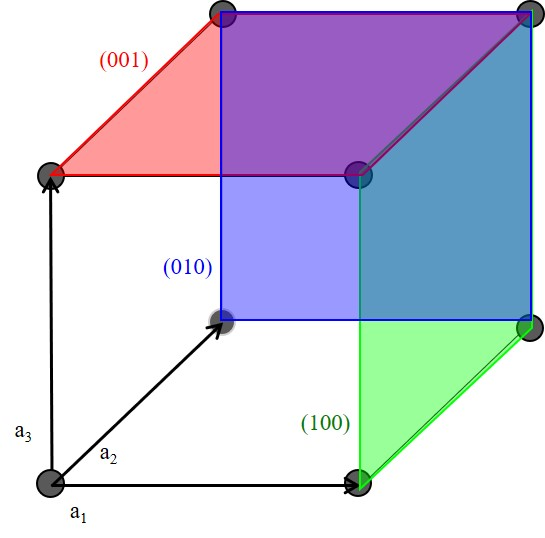
\includegraphics[clip, width=4.5cm]{a1.jpg}
   \hspace{2cm} (a)
  \end{minipage}

  \begin{minipage}{0.5\hsize}
   \centering
   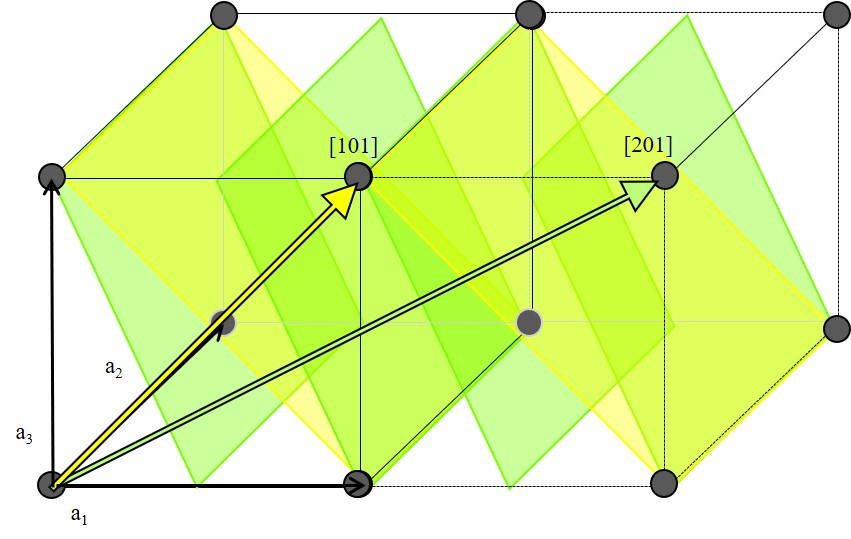
\includegraphics[clip, width=6cm]{a2.jpg}
   \hspace{2cm} (b)
  \end{minipage}

 \end{tabular}
 \caption{結晶面の概形.}
 \label{a1}

\end{figure}

\newpage
\subsection{逆格子}
結晶の構造においては、単位格子が空間的に繰り返す周期性がある。ここで、並進操作$\bm{r}\to\bm{r+R}$に対し不変となるベクトル
\begin{equation}
\bm{R}=n_a\bm{a_1}+n_b\bm{a_2}+n_c\bm{a_3}
\nonumber
\end{equation}
が存在する。$\bm{R}$を実格子ベクトルと呼ぶ。ここで、結晶と同様の周期性を持つ関数$\phi(\bm{r})=\phi(\bm{r+R})$を波数ベクトル$\bm{G}$でフーリエ展開すると、
\begin{equation}
  \phi(\bm{r})=\sum_{\bm{G}}\phi_{\bm{G}}e^{i\bm{G\cdot r}}
  \label{r}
\end{equation}

\begin{equation}
  \phi(\bm{r+R})=\sum_{\bm{G}}\phi_{\bm{G}}e^{i\bm{G\cdot (r+R)}}
  \label{r+R}
\end{equation}

となる。ここで、式(\ref{r})と式(\ref{r+R})は等しいため、$\bm{R}$と$\bm{G}$は
\begin{equation}
e^{i\bm{G\cdot R}}=1\leftrightarrow\bm{G\cdot R}=2n\pi
  \label{GR}
\end{equation}
を満たさなければならない。このような$\bm{G}$を
\begin{equation}
\bm{G}=h\bm{b_1}+k\bm{b_2}+l\bm{b_3}
\nonumber
\end{equation}
と定義する。$hkl$は回折指数である。$\bm{G}$を逆格子ベクトルと呼び、$(長さ)^{-1}$の次元を持つ。この時、$\bm{a}_j$と$\bm{b}_k$の間には、
\begin{equation}
\bm{a}_j\cdot\bm{b}_k=\delta_{jk}
\end{equation}
\begin{numcases}
{}
\delta_{jk}=0(j\neq k)\\
\delta_{jk}=2\pi(j=k)
\nonumber
\end{numcases}
の関係がある。ここで、$|a_1|=|a_2|=|a_3|$かつ$|b_1|=|b_2|=|b_3|$のとき、$|b_j|=\frac{1}{|a_j|}$である。
$l=0$のときの、実格子空間と逆格子空間の簡単な対応を図\ref{kousi}に示す。
\begin{figure}[htb]
 \centering
 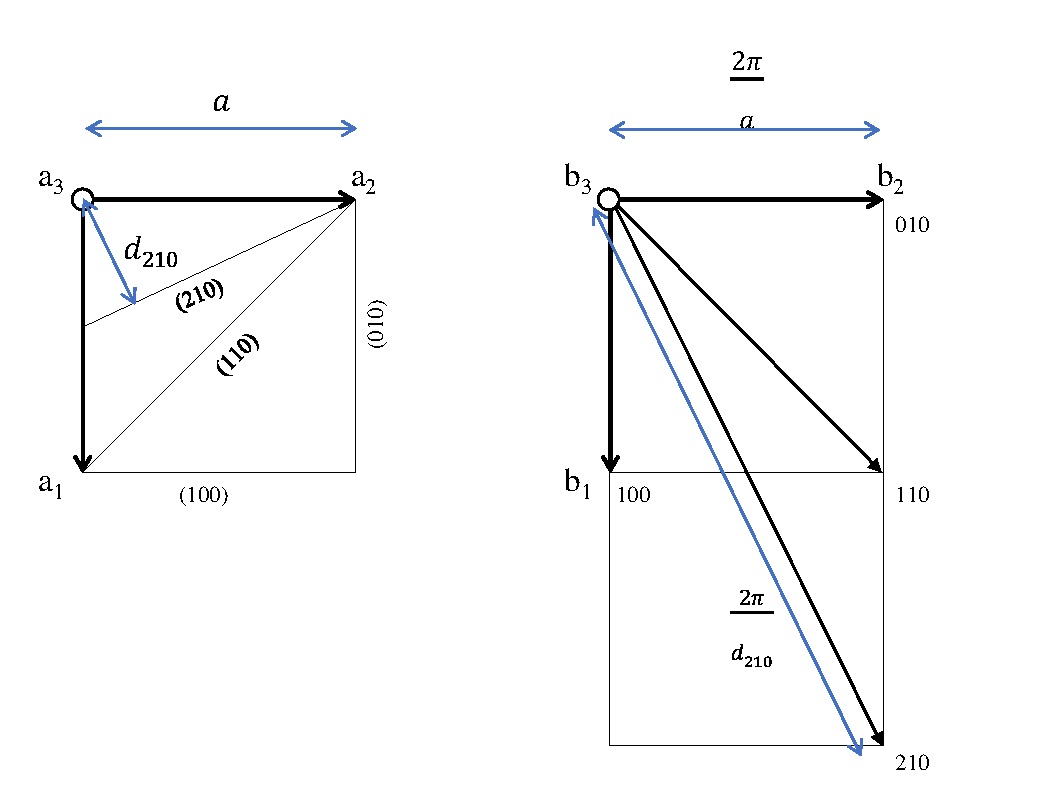
\includegraphics[clip,width=10cm]{kousi.eps}
 \caption{実格子と逆格子の関係.}
 \label{kousi}
\end{figure}

\newpage
左が実格子空間、右が逆格子空間である。$hkl=210$を見ると、逆格子ベクトル[210]は、実格子における(210)と垂直である。また、$\bm{G}_{hkl}$方向の結晶面の間隔$d_{hkl}$は
\begin{equation}
  d_{hkl}=\frac{2\pi}{|\bm{G}_{hkl}|}\times \mathrm{gcd}(h,k,l)
\end{equation}
と表せる。gcd$(h,k,l)$は$(h,k,l)$の最大公約数である。最大公約数が1であるとき、つまり$(h,k,l)$の組が互いに素であるとき、回折指数$hkl$とミラー指数$(h,k,l)$は一致する。



\newpage
\subsection{回折条件}
実格子空間でのX線の回折の条件を考える。X線がある結晶面によって散乱を起こすときの光路を図\ref{hasuu}(a)に示す。入射光と結晶面の角度を$\theta$、結晶面の間隔を$d$としたとき、この時、2つの光の光路差は$2d\sin\theta$である。散乱前後で光の波長が変化しないとき、この光路差がX線の波長の整数倍であれば、散乱光は強め合う。よって、実格子空間におけるX線の回折の条件は
\begin{equation}
 2d\sin\theta=n\lambda
 \label{bragg}
\end{equation}
となる。この条件をBragg条件と呼ぶ。


また、逆格子空間でのX線の回折の条件を考える。入射X線の波数ベクトルを$\bm{k_0}$、散乱X線の波数ベクトルを$\bm{k}$とする。逆格子空間におけるX線の散乱を図\ref{hasuu}(b)に示す。
$\bm{k_0}$が逆格子空間の原点を向くベクトルだと考えると、$\bm{k}$の終着点は$\bm{k_0-k}$で表せる(これを散乱ベクトルと呼ぶ)。ここで、散乱ベクトルが逆格子ベクトル$\bm{G}_{hkl}$と等しいとき、つまり、散乱X線の波数ベクトルの終点が逆格子空間の格子点に等しいとき、回折が起きる。したがって、逆格子空間におけるX線の回折の条件は、
\begin{equation}
 \bm{k-k_0}=\bm{G}_{hkl}
 \label{laue}
\end{equation}
となる。この条件をLaue条件と呼ぶ。
\begin{figure}[ht]
 \centering
 \begin{tabular}{c}

  \begin{minipage}{0.5\hsize}
   \centering
   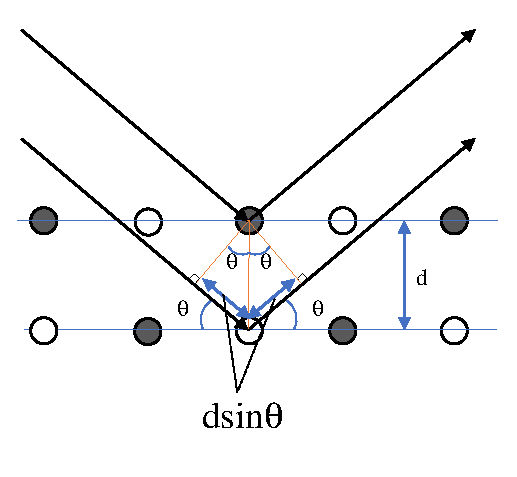
\includegraphics[clip, width=4.5cm]{dsinq.eps}
   \hspace{2cm} (a)
  \end{minipage}

  \begin{minipage}{0.5\hsize}
   \centering
   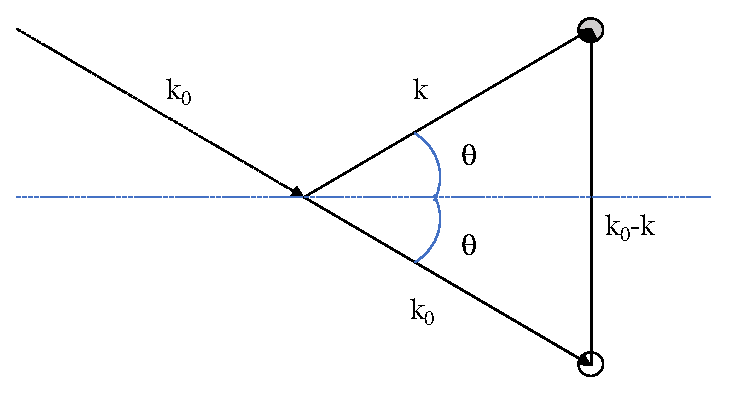
\includegraphics[clip, width=6cm]{hasuu.eps}
   \hspace{2cm} (b)
  \end{minipage}

 \end{tabular}
 \caption{X線の散乱.}
 \label{hasuu}

\end{figure}


\if0
\newpage%ここいる?
図\ref{hasuu}を見ると、入射X線と散乱X線のなす角が$2\theta$であることがわかる。ここで、Thomson散乱を考えるとき、散乱前後で波数は変化しないので、$\bm{|k_0|=|k|}$である。よって、
\begin{equation}
 \bm{2|k|}\sin\theta=|\bm{G}_{hkl}|
 \nonumber
\end{equation}
である。これに、$\bm{|k|}=\frac{2\pi}{\lambda}$と、$|\bm{G}_{hkl}|=\frac{2\pi}{d_{hkl}}$を代入すると、
\begin{equation}
 2\cdot\frac{2\pi}{\lambda}\sin\theta=\frac{2\pi}{d_{hkl}}
 \nonumber
\end{equation}
が導ける。これを変形するとBraggの条件と一致するので、式(\ref{bragg})と式(\ref{laue})は等価である。
\fi

\newpage
\subsection{X線回折}%ここいる?
X線は電磁波であり、結晶にX線を入射したとき、X線は構成原子の原子核と電子によって散乱される。荷電粒子による電磁波の散乱には、散乱波の波長が元の波長から変化しないThomson散乱と、散乱はの波長が元の波長よりも長くなるCompton散乱の2種類がある。Thomson散乱は干渉性散乱、Compton散乱は非干渉性散乱である。結晶による回折においては、干渉性散乱のみを考えればよいので、Thomson散乱のみを考える。Thomson散乱において、散乱断面積は散乱体の質量の自乗に反比例するため、原子によるX線の散乱は電子による散乱に比べ十分小さくなる。ここから、X線は電子によって散乱されるとみなせる。
図\ref{sanran}のように、密度$\rho(\bm{r})$で空間分布した電子雲によってX線が散乱される場合を考える。
\begin{figure}[htb]
 \centering
 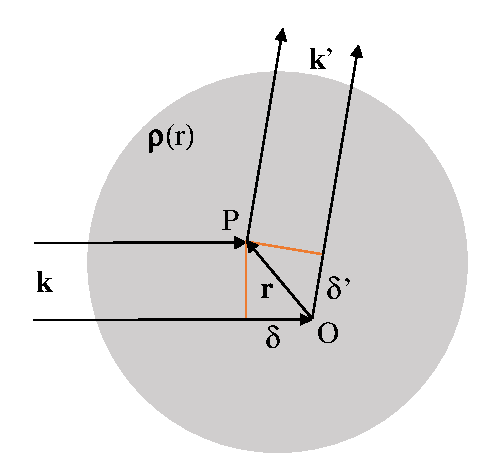
\includegraphics[clip,width=5cm]{sanran.eps}
 \caption{電子雲によるX線の散乱.}
 \label{sanran}
\end{figure}

電子雲に平面波のX線が入射して、原点Oと点Pで波数$\bm{k}$から$\bm{k}'$に散乱された時、位相差は
\begin{equation}
  \delta_1+\delta_2=\bm{(-k\cdot r)+(k'\cdot r)}=K\cdot r
\end{equation}
と表せる(散乱ベクトル$\bm{K=k'-k}$を定義した)。
この時、ある散乱先$\bm{r'}$における散乱X線の重ね合わせは
\begin{equation}
  A\rho\bm{(0)}e^{i(\bm{k'\cdot r'})}+  A\rho\bm{(r)}e^{i(\bm{k'\cdot r'+\delta_1+\delta_2})}=A[\rho\bm{(0)}e^{i(\bm{K\cdot 0})}+\rho\bm{(r)}e^{i(\bm{K\cdot r})}]e^{i(\bm{k'\cdot r'})}
\end{equation}
となる(A:定数)。ここで、右辺の[]内の項は、点O、Pで散乱されたX線の振幅に等しい。よって、電子雲全体での散乱振幅は、
\begin{equation}
  f=\int\rho(\bm{r})e^{i\bm{K\cdot r}}d\bm{r}
  \label{insi}
\end{equation}
に比例することがわかる。

\newpage
ところで、$\rho(\bm{r})$は、結晶の構成原子それぞれの電子密度の和
\begin{equation}
  \rho(\bm{r})=\sum_{\bm{R}}\sum_j\rho_j(\bm{r-[R+}\bm{r}_j])
\end{equation}
で表せる($\bm{r}_j$:結晶中のj番目の原子の位置ベクトル)。これを用いて式(\ref{insi})を変形すると、
\begin{equation}
  \begin{split}
  f&=\int\rho(\bm{r})=\sum_{\bm{R}}\sum_j\rho_j(\bm{r-R-}\bm{r}_j)e^{i\bm{K\cdot r}}d\bm{r}\\
  &=\sum_{\bm{R}}e^{i\bm{K\cdot R}}\sum_je^{i\bm{K}\cdot\bm{r}_j}\int\rho_j(\bm{r-R-}\bm{r}_j)e^{i\bm{K\cdot (\bm{r-R-}\bm{r}_j)}}d\bm(r)\\
  &=\sum_{\bm{R}}e^{i\bm{K\cdot R}}\sum_jf_je^{i\bm{K}\cdot\bm{r}_j}
\end{split}
\end{equation}
となる。式(\ref{insi})より、$\int\rho_j(\bm{r-R-}\bm{r}_j)e^{i\bm{K\cdot (\bm{r-R-}\bm{r}_j)}}=f_j$とした。結晶全体の散乱の和を$\sum_{\bm{R}}e^{i\bm{K\cdot R}}\equiv G(\bm{K})$、単位格子中の散乱の和を$\sum_jf_je^{i\bm{K}\cdot\bm{r}_j}\equiv F(\bm{K})$と定義する。この時、散乱X線の強度は
\begin{equation}
  {|f|}^2={|G\bm{(K)}|^2}{|F\bm{(K)}|^2}
  \label{kyoudo}
\end{equation}に比例する。
$\bm{a_1}、\bm{a_2}、\bm{a_3}$方向の格子数を$N_a、N_b、N_c$としたとき、$|G(\bm{K})|^2$は等比級数として計算でき、
\begin{equation}
  |G(\bm{K})|^2=\frac{\sin^2(N_a\bm{K}\cdot\bm{a}_1/2)}{\sin^2(\bm{K}\cdot\bm{a}_1/2)}\frac{\sin^2(N_b\bm{K}\cdot\bm{a}_2/2)}{\sin^2(\bm{K}\cdot\bm{a}_2/2)}\frac{\sin^2(N_c\bm{K}\cdot\bm{a}_3/2)}{\sin^2(\bm{K}\cdot\bm{a}_3/2)}
\end{equation}
と表せる。これをLaue関数と呼ぶ。$|G(\bm{K})|^2$は、波数ベクトル$\bm{K}$と各方向成分$\bm{a_1}、\bm{a_2}、\bm{a_3}$の内積が
\begin{equation}
  \bm{K}\cdot\bm{a}_1=2\pi h、\bm{K}\cdot\bm{a}_2=2\pi k、\bm{K}\cdot\bm{a}_3=2\pi l、
\end{equation}
のとき、つまり$\bm{K}$がLaue条件を満たすとき有限の値をとり、それ以外の場合はほぼ0である。%余力あれば例を示す

$G(\bm{K})$がLaue関数であることから、$F(\bm{K})$について、$\bm{K}=\bm{G}_{hkl}$として計算できる。よって、
\begin{equation}
\begin{split}
    F_{hkl}&=\sum_jf_je^{i\bm{G}_{hkl}\cdot\bm{r}_j}\\
    &=\sum_jf_je^{2\pi i(h\bm{b_1}+k\bm{b_2}+l\bm{b_3})}
\end{split}
\end{equation}
となる。$F_{hkl}$を結晶構造因子と呼ぶ。結晶構造因子はLaue関数と同様、特定の条件を満たすとき有限の値をとり、それ以外の場合は0である。したがって、Laue条件を満たしていても、$F_{hkl}=0$のとき回折は観測されない。これを消滅則と呼ぶ。格子の形状によって、有限の値をとる条件が異なるため、結晶構造の解析の際に有用である。

\newpage
\subsection{NaClの結晶構造}
NaCl結晶は、NaCl型構造をとる。NaClの構造の概形を図\ref{nacl}に示す。

\begin{figure}[htb]
 \centering
 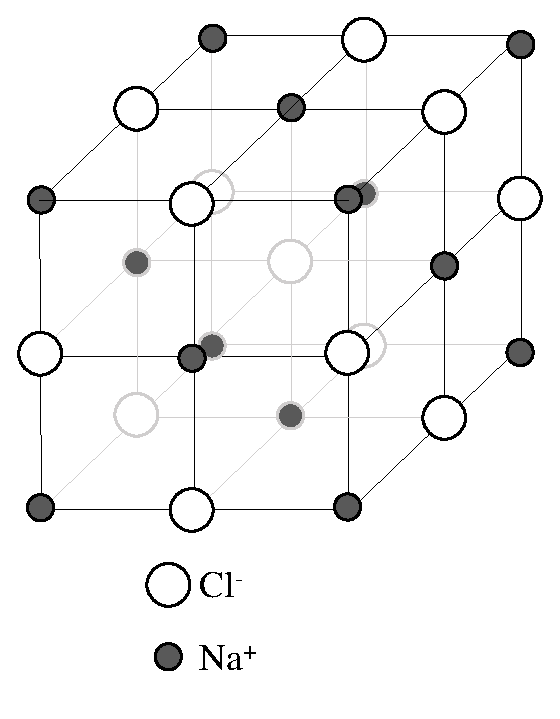
\includegraphics[clip,width=7cm]{nacl.eps}
 \caption{NaClの結晶構造.}
 \label{nacl}
\end{figure}

NaCl結晶は、Naサイトの面心立方格子とClサイトの面心立方格子が入れ子になった構造になっている。NaCl結晶における結晶構造因子$F_{hkl}$を考える。
単位格子において、橙の矢印のように単位ベクトル$\bm{a}_i(i=1,2,3)$($|a_1|=|a_2|=|a_3|$)の原点をとると、$\mathrm{Na}$原子は
\begin{equation}
  \bm{r}_1=0,\bm{r}_2=\frac{1}{2}\bm{a}_1+\frac{1}{2}\bm{a}_2,\bm{r}_3=\frac{1}{2}\bm{a}_2+\frac{1}{2}\bm{a}_3,\bm{r}_4=\frac{1}{2}\bm{a}_3+\frac{1}{2}\bm{a}_1
\end{equation}
の4つの非等価な位置に存在している。よって、$\mathrm{Na}$原子による原子散乱因子を$f_{\mathrm{Na}}$とすると、$F_{\mathrm{Na}}$は
\begin{equation}
  \begin{split}
  F_{\mathrm{Na}}&=\sum_{j=1}^4f_{\mathrm{Na}}e^{i\bm{G}_{hkl}\cdot\bm{r}_j}\\
  &=f_{\mathrm{Na}}(1+e^{i\pi(h+k)}+e^{i\pi(k+l)}+e^{i\pi(l+h)})
\end{split}
\end{equation}
となる。$\mathrm{Cl}$原子においては、青の矢印のように$\bm{r}=\frac{1}{2}\bm{a}_1+\frac{1}{2}\bm{a}_2+\frac{1}{2}\bm{a}_3$の位置から考える。Cl原子原子による原子散乱因子を$f_{\mathrm{Cl}}$とすると、$F_{\mathrm{Cl}}$は
\if0%Clの原子位置
\begin{equation}
  \begin{split}
  \bm{r}_1=\frac{1}{2}\bm{a}_1+\frac{1}{2}\bm{a}_2+\frac{1}{2}\bm{a}_3\\
  \bm{r}_2=\bm{a}_1+\bm{a}_2+\frac{1}{2}\bm{a}_3\\
  \bm{r}_3=\frac{1}{2}\bm{a}_1+\bm{a}_2+\bm{a}_3\\
  \bm{r}_4=\bm{a}_1+\frac{1}{2}\bm{a}_2+\bm{a}_3
\end{split}
\end{equation}
\fi

\begin{equation}
  F_{\mathrm{Cl}}=f_{\mathrm{Cl}}\cdot e^{i\pi(h+k+l)}(1+e^{i\pi(h+k)}+e^{i\pi(k+l)}+e^{i\pi(l+h)})
\end{equation}
となる。NaCl結晶における結晶構造因子は、$F_{\mathrm{Na}}$と$F_{\mathrm{Cl}}$の合計なので、$F_{\mathrm{hkl}}$は
\begin{equation}
  F_{\mathrm{hkl}}=(f_{\mathrm{Na}}+f_{\mathrm{Cl}}\cdot e^{i\pi(h+k+l)})(1+e^{i\pi(h+k)}+e^{i\pi(k+l)}+e^{i\pi(l+h)})
\end{equation}
となる。NaCl結晶における$F_{\mathrm{hkl}}$の消滅則は、$hkl$の組み合わせから、
\begin{subequations}
\begin{equation}
F_{hkl}=\begin{cases}
4(f_{\mathrm{Na}}+f_{\mathrm{Cl}}) & h,k,lがすべて偶数 \\
4(f_{\mathrm{Na}}-f_{\mathrm{Cl}}) & h,k,lがすべて奇数\\
0 & その他
\end{cases}
\end{equation}
\end{subequations}
となる。
\newpage
\subsection{$2\theta/\theta$法}

X線回折装置の概略図を図\ref{thetatheta}に示す。試料台に平行な結晶面と入射X線のなす角(入射角)が$\theta$のとき、試料に平行な結晶面と散乱X線のなす角も$\theta$となる。$\theta$の値を変える時、つまりX線源を動かす時、回折光が観測できるように光検出器も同時に動かす観測方法を$2\theta/\theta$法と呼ぶ。試料が単結晶の場合は、図\ref{thetatheta}(a)のように、試料台に平行な面は$(h,k,l)=(0,0,n)$の面のみであるため、Laue条件と消滅則を満たす$(0,0,n)$面からの回折のみが観測できる。試料が粉末の場合は、図\ref{thetatheta}(b)のように、$(h,k,l)=(0,0,n)$以外にも試料台に平行な面があるため、Laue条件と消滅則を満たせば、様々な$(h,k,l)$からの回折が観測できる。


\begin{figure}[ht]
 \centering
 \begin{tabular}{c}

  \begin{minipage}{0.5\hsize}
   \centering
   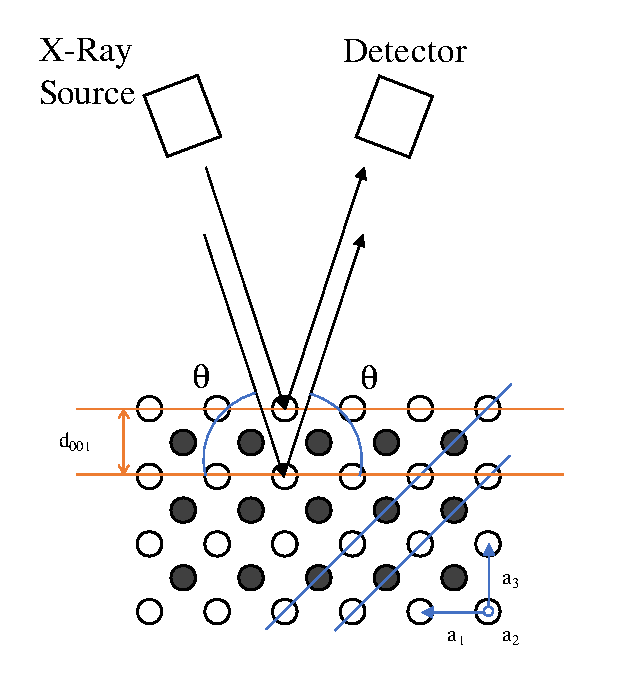
\includegraphics[clip, width=5.3cm]{2theta.eps}
   \hspace{2cm} (a)
  \end{minipage}

  \begin{minipage}{0.5\hsize}
   \centering
   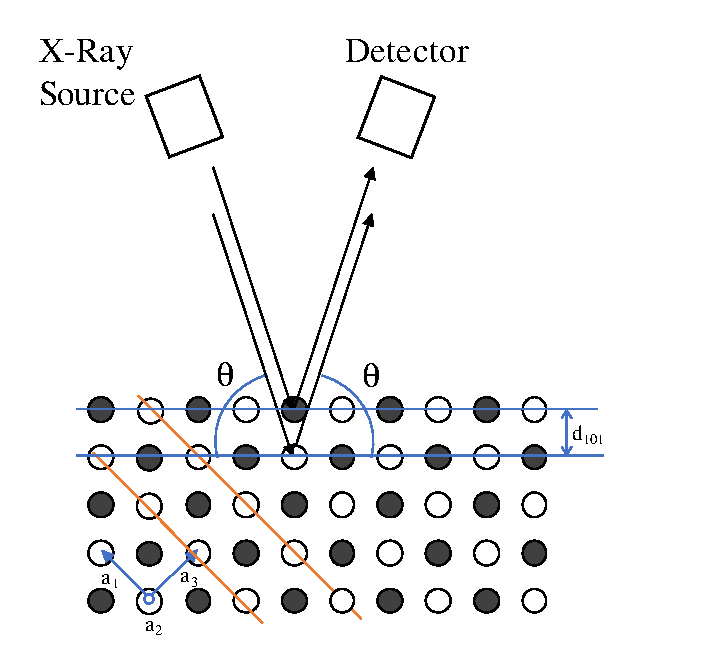
\includegraphics[clip, width=6cm]{2theta3.eps}
   \hspace{2cm} (b)
  \end{minipage}

 \end{tabular}
 \caption{X線回折装置概略図.}
 \label{thetatheta}

\end{figure}

\newpage
\subsection{NaCl粉末の回折パターン}

NaCl粉末の、$2\theta$の値が90よりも小さいときの回折パターンを表\ref{data}に示す。この表は、入射光と回折光のなす角が$2\theta$の時、どの$(h,k,l)$面が試料台に平行で、どの程度の強度で回折光が観測できるかを示している。また、$(h,k,l)$面における面間隔も示している。実験データの解析のおいては、この表のデータを参照する。

\begin{table}[htbp]
 \begin{center}
  \caption{NaCl粉末の回折パターン\cite{powder}.}
  \begin{tabular}{|r|r|r|r|r|r|}  \hline
                           & \multicolumn{3}{c|}{} &   &                                \\
   $2\theta(\mathrm{deg})$ & h                     & k & l & Intensity & d-spacing [nm] \\  \hline \hline
   26.886                  & 1                     & 1 & 1 & 10        & 0.3312         \\
   31.145                  & 2                     & 0 & 0 & 99        & 0.2869         \\
   44.629                  & 2                     & 2 & 0 & 61        & 0.2028         \\
   52.878                  & 3                     & 1 & 1 & 3         & 0.173          \\
   55.426                  & 2                     & 2 & 2 & 19        & 0.1656         \\
   64.959                  & 4                     & 0 & 0 & 8         & 0.1434         \\
   71.633                  & 3                     & 3 & 1 & 2         & 0.1316         \\
   73.797                  & 4                     & 2 & 0 & 19        & 0.1283         \\
   82.251                  & 4                     & 2 & 2 & 13        & 0.1171         \\
   88.472                  & 5                     & 1 & 1 & 2         & 0.1104         \\ \hline
  \end{tabular}
  \label{data}
 \end{center}
\end{table}

\newpage
\section{NaCl粉末及び単結晶の回折パターンの観測方法}

NaCl粉末及び単結晶の回折パターンを、X線回折装置"SmartLab"を用いて、$2\theta/\theta$法で観測した。$\mathrm{SmartLab}$の構造を図\ref{smartlab}に示す。


\begin{figure}[htb]
 \centering
 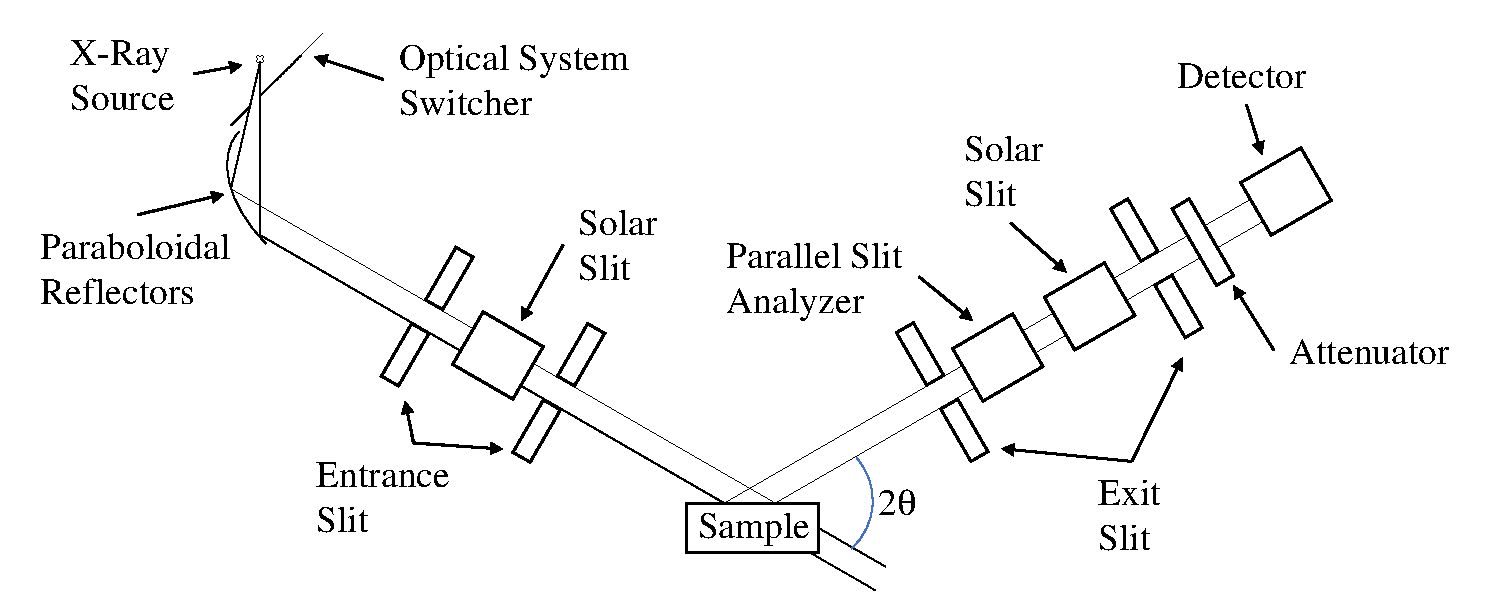
\includegraphics[clip,width=12cm]{XRD.eps}
 \caption{SmartLabの内部構造.}
 \label{smartlab}
\end{figure}

X線源から放射された光をNaCl粉末及び単結晶に照射し、光検出器で回折光を観測した。X線源のターゲット金属はCuである。特性X線のうち、波長が1.543 \AA の$K_\alpha$線と、1.392 \AA の$K_\beta$線を用いた。X線源から等方的に放射された光を、放物面人工多層膜ミラーを用いて単色化・平行化し、2枚の入射スリットとソーラースリットを用いて発散を制限した。2枚の出射スリットとソーラースリットを用いて、試料からの回折光の発散を制限した。アッテネーターを用いて、光検出器に入射する光を減衰させた。PSA(平行スリットアナライザー)を用いて分解能を決定した。$2\theta$は入射光と出射光のなす角である。表\ref{exp}の実験条件の下、試料ごとに$2\theta$を変えてゆき、回折パターンを測定した。試料はNaCl粉末とNaCl単結晶の2種類である。単結晶試料の寸法を図\ref{size}に示す。

\begin{table}[ht]
 \centering
 \caption{実験条件.}
 \begin{tabular}{lc}\hline
  \multicolumn{2}{c}{実験条件}          \\ \hline
  入射スリット     & 1 mm               \\
  出射スリット     & 1 mm               \\
  ソーラースリット & 0.5 deg            \\
  X線波長          & 1.543 \AA、1.392 \AA \\\hline
 \end{tabular}
 \label{exp}
\end{table}

\begin{figure}[htb]
 \centering
 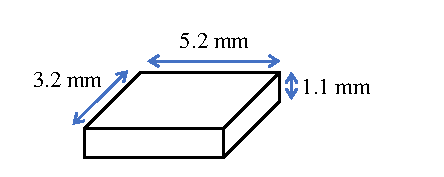
\includegraphics[clip,width=9cm]{bulk.eps}
 \caption{NaCl単結晶の寸法.}
 \label{size}
\end{figure}


\newpage
実験に用いた単結晶は、縦3.2 mm、横5.2 mm、高さ1.1 mmの直方体のものである。この結晶を、最も面積の広い面を下にして試料台に設置した。

\newpage
\section{NaCl粉末及び単結晶の回折パターンの解析}


\subsection{NaCl粉末}

NaCl粉末における回折パターンを図\ref{powder}に示す。

\begin{figure}[htb]
 \centering
 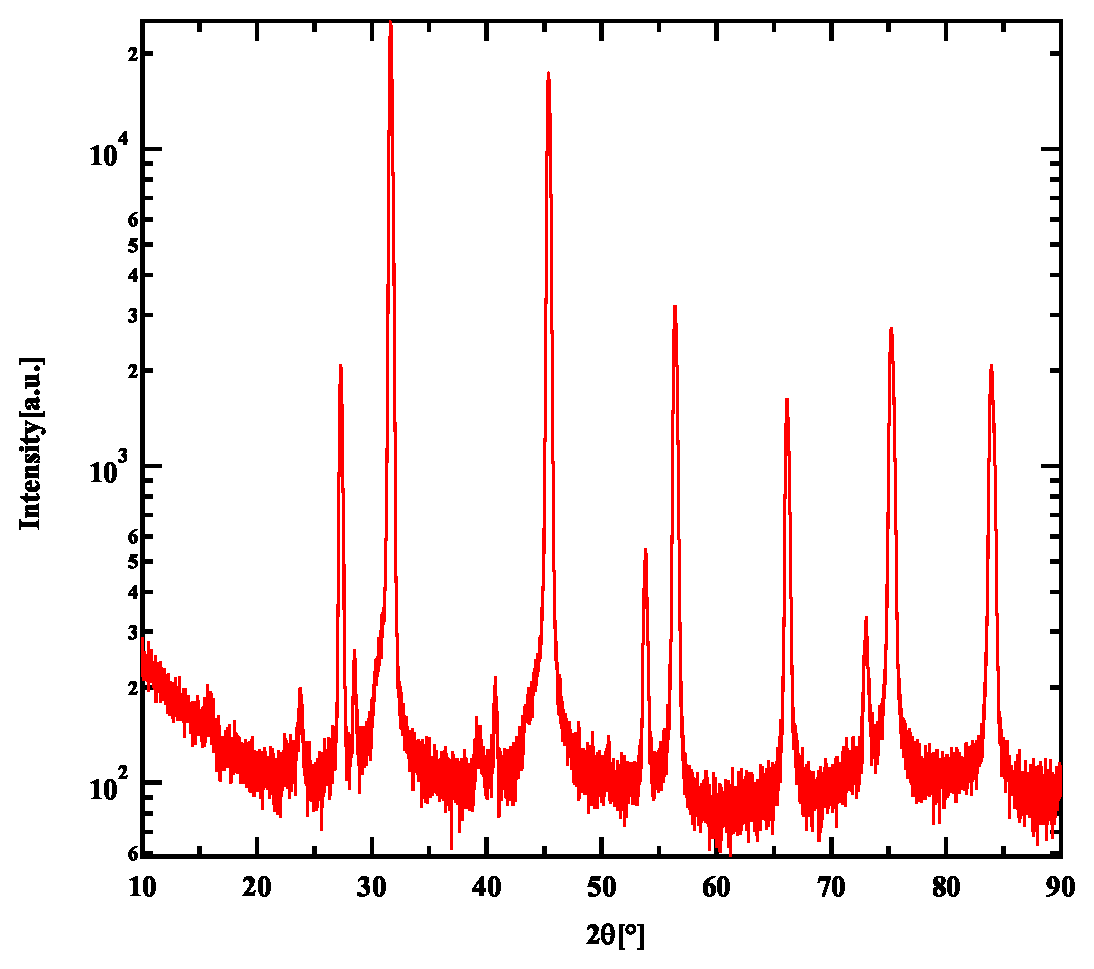
\includegraphics[clip,width=7cm]{FigPowder.eps}
 \caption{NaCl粉末の回折パターン.}
 \label{powder}
\end{figure}

横軸は入射光と回折光のなす角、縦軸は回折強度である。グラフから、鋭いピークが複数見られる。これらのピークのうち、頂点における$2\theta$が、表\ref{data}の値と近いものだけを抜き出したものを表\ref{pow}に示す。

\begin{table}[htbp]
 \begin{center}
  \caption{NaCl粉末の格子定数.}
  \begin{tabular}{|c|r|c|lll|c|}  \hline
   $2\theta[\mathrm{deg}]$ & \multicolumn{1}{c|}{$2\theta[\mathrm{rad}]$} & $G_{m}$     & h & k & l & a           \\ \hline  \hline
   27.306 & 0.4766  & 1.9223 & 1 & 1 & 1 & 5.6583\\
   31.646 & 0.5523  & 2.2206 & 2 & 0 & 0 & 5.6561\\
   45.397 & 0.7923  & 3.1427 & 2 & 2 & 0 & 5.6521\\
   53.828 & 0.9395  & 3.6865 & 3 & 1 & 1 & 5.6500\\
   56.419 & 0.9847  & 3.8497 & 2 & 2 & 2 & 5.6510\\
   66.178 & 1.1550  & 4.4462 & 4 & 0 & 0 & 5.6498\\
   73.041 & 1.2748  & 4.8466 & 3 & 3 & 1 & 5.6480\\
   75.259 & 1.3135  & 4.9724 & 4 & 2 & 0 & 5.6482\\
   83.979 & 1.4657  & 5.4484 & 4 & 2 & 2 & 5.6468\\\hline
  \end{tabular}
  \label{pow}
 \end{center}
\end{table}

\newpage
逆格子ベクトルの大きさ$G_{m}$は
\begin{equation}
 G_m=\frac{4\pi}{\uplambda}\sin\theta
 \label{gyakukousi}
\end{equation}
で計算した。$\uplambda$は、今回は$K_\alpha$線の波長である1.543 \AA を用いた。格子定数$a$は、$G_{m}$から
\begin{equation}
 a=\frac{2\pi}{G_m}\sqrt{h^2+k^2+l^2}
 \label{kousiteisuu}
\end{equation}
で計算した。各$\theta$におけるaの平均をとって、格子定数は
\begin{equation}
 \nonumber
 a=5.6511
 \label{complete}
\end{equation}
と求まった。

\newpage
\subsection{NaCl単結晶}



NaCl単結晶における回折パターンを図\ref{bulk}に示す。

\begin{figure}[htb]
 \centering
 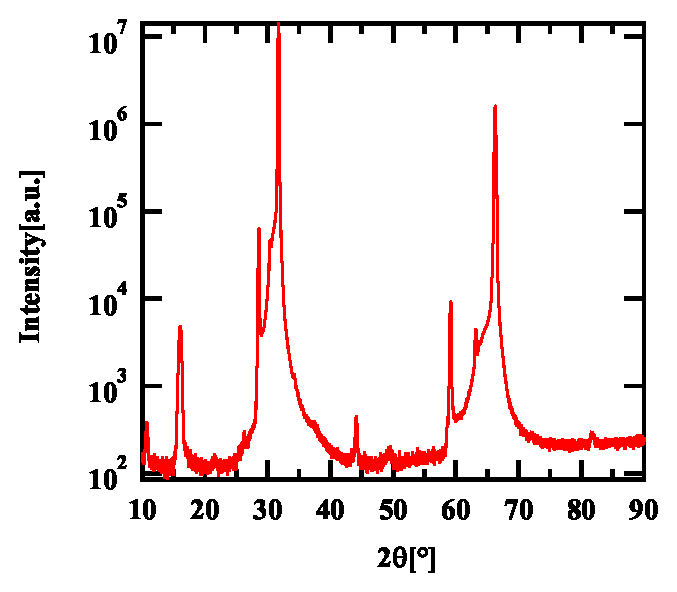
\includegraphics[clip,width=9cm]{FigBulk.eps}
 \caption{NaCl単結晶の回折パターン.}
 \label{bulk}
\end{figure}

横軸はAの回転角、縦軸は回折強度である。グラフから、鋭いピークが複数見られる。$2\theta/\theta$法を用いた単結晶のX線回折測定では、(001)面に平行な面での回折しか観測できないため、$K_\alpha$線及び$K_\beta$線の二つのX線による回折が観測できる。したがって、どのピークが、どのX線による回折を示しているのか判断ができない。$2\theta/\theta$法を用いた単結晶のX線回折測定では、(001)面に平行な面での回折しか観測できないことを利用し、(h,k,l)=(0,0,2n)となるように回折指数をとり、粉末試料で得た格子定数から$2\theta$を逆算した。その結果を表\ref{gyakusan}に示す。

\begin{table}[htbp]
 \begin{center}
  \caption{2$\theta$の見積もり.}
  \begin{tabular}{|c|c|c|c|c|}\hline
   $a$        & $\lambda$ & l & $\theta$[rad] & 2$\theta$[deg] \\  \hline  \hline
   5.6511 & 1.39 & 2 & 0.2485 & 28.478\\
 5.6511 & 1.54 & 2 & 0.2760& 31.628\\
 5.6511 & 1.39 & 4 & 0.5143 & 58.936\\
 5.6511 & 1.54 & 4 & 0.5764 & 66.053\\
 \hline
  \end{tabular}
  \label{gyakusan}
 \end{center}
\end{table}

\newpage
表\ref{gyakusan}から、$K_\alpha$線及び$K_\beta$線由来の、(0,0,2n)面による回折角が見積もれた。図\ref{bulk}のピークのうち、頂点における2$\theta$が、表\ref{gyakusan}に近いものだけを抜き出したものを表\ref{crystal}に示す。

\begin{table}[htbp]
 \begin{center}
  \caption{NaCl単結晶の格子定数.}
  \begin{tabular}{|c|c|c|c|ccc|c|c|c|}  \hline
   $2\theta[\mathrm{deg}]$ & $2\theta[\mathrm{rad}]$ & $G_{m\beta}$       & $G_{m\alpha}$      & h & k & l & $a_\beta$          & $a_\alpha$         \\   \hline  \hline
   28.598 & 0.4991 & 2.2317 & \sout{2.0154} & 0 & 0 & 2 & 5.6279 & \sout{6.232}\\
 31.739 & 0.5540 & \sout{2.4709} & 2.2313 & 0 & 0 & 2 & \sout{5.0832} & 5.6289\\
  59.173 & 1.0328 & 4.4614 & \sout{4.0289} & 0 & 0 & 4 & 5.6305 & \sout{6.2350}\\
  66.28 & 1.1568 & \sout{4.9398} & 4.4610 & 0 & 0 & 4 & \sout{5.0852} & 5.6311\\
  \hline
  \end{tabular}
  \label{crystal}
 \end{center}
\end{table}

%単結晶においては、(001)面に平行な面での回折のみが見られることから、$K_\beta$線による回折も観測できる。そのため、各回折指数hklにおいて、2つの格子定数が計算できる。この逆算から、特性X線$K_\alpha$と$K_\beta$による1次と2次の回折角が得られた。それを図\ref{kakb}に示す。
逆格子ベクトルの大きさ$G_m$および格子定数$a$は、NaCl粉末と同様の方法で計算した。$\lambda$は表\ref{gyakusan}のように、$K_\alpha$線による回折は1.543 \AA 、$K_\beta$線による回折は1.392 \AA を用いた。各$\theta$における$a$の平均をとって、格子定数は
\begin{equation}
 \nonumber
 a=5.6296
 \label{complete2}
\end{equation}
と求まった。

\if0
図\ref{crystal}ににおける$K_\alpha$線と$K_\beta$線による回折のピークを、直線でつないだものを図\ref{kakb}に示す。

 \begin{figure}[htb]
  \centering
  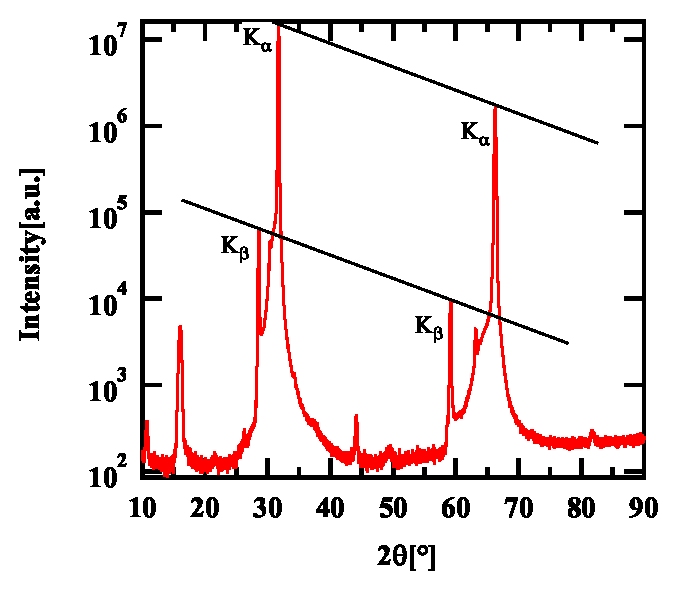
\includegraphics[clip,width=9cm]{kakb.eps}
  \caption{NaCl結晶の回折パターン.}
  \label{kakb}
 \end{figure}

片対数グラフにおいて、$K_\alpha$線と$K_\beta$線のどちらも、回折角が大きくなると回折強度が小さくなっていることが分かる。
\fi
また、図\ref{bulk}から、回折角が大きくなると、回折強度が小さくなっていることがわかる。
式(\ref{kyoudo})より、回折光の強度は${|f|}^2={|G\bm{(K)}|^2}{|F\bm{(K)}|^2}$に比例する。今回の回折面は$(0,0,2)$面及び$(0,0,4)$面である。$h=0、k=0$であるため、
\begin{equation}
  |G(\bm{K})|^2=\frac{\sin^2(N_c\bm{K}\cdot\bm{a}_3/2)}{\sin^2(\bm{K}\cdot\bm{a}_3/2)}
\end{equation}
となる。この時、$|G(\bm{K})|^2$の極大値は$N_c^2$に比例するが、$N_c$の値は$l$方向の格子の数であるから、$|G(\bm{K})|^2$は変化しない。$F(\bm{K})$は
\begin{equation}
  F_{hkl}=4(f_{\mathrm{Na}}+f_{\mathrm{Cl}})
\end{equation}
となる。この式における原子散乱因子$f_{\mathrm{Na}}+f_{\mathrm{Cl}}$は図\ref{atomic}のように$\frac{\sin\theta}{\lambda}$依存性を持つ\cite{atom}。X線は原子でなく電子によって散乱されるため、X線波長$\lambda$が一定の時、回折角$\theta$が大きくなると、個々の電子による散乱X線の位相差も大きくなる。そのため、原子散乱因子は減少する。また、回折角$\theta$が一定の時、X線波長$\lambda$が短くなると、波長に対しX線の光路差が大きくなるため、原子散乱因子が減少する。回折光の強度は原子散乱因子の自乗に比例するため、図\ref{bulk}において、回折角が大きくなると回折強度が小さくなっている。

\begin{figure}[htb]
 \centering
 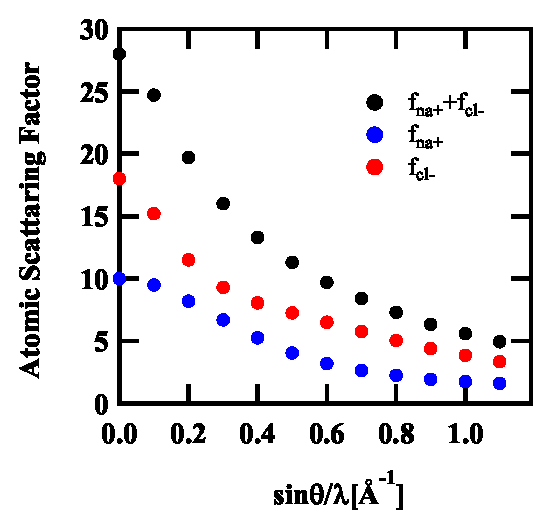
\includegraphics[clip,width=7cm]{atomic.eps}
 \caption{原子散乱因子の$\theta$及び波長依存性.}
 \label{atomic}
\end{figure}


\if0%逆格子空間で議論しよう!のはなし
このことについて、図\ref{laue2}のような逆格子空間における回折を用いて考える。
\begin{figure}[htb]
 \centering
 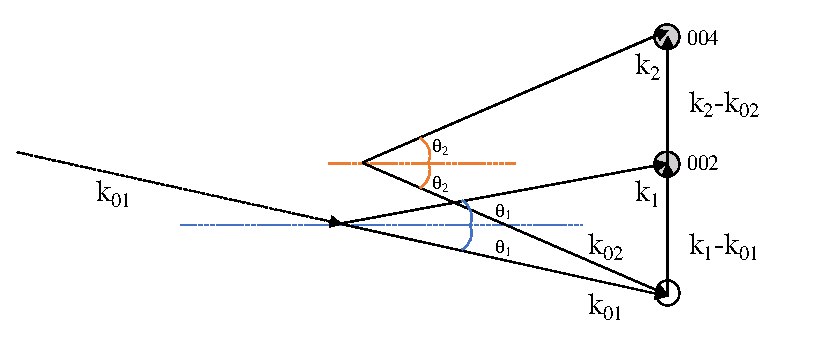
\includegraphics[clip,width=9cm]{laue2.eps}
 \caption{逆格子空間における回折.}
 \label{laue2}
\end{figure}

\newpage
式(\ref{kyoudo})より、回折光の強度は${|f|}^2={|G\bm{(K)}|^2}{|F\bm{(K)}|^2}$に比例する。今回、$(h,k,l)$はすべて偶数であるため、どちらの回折においても
\begin{equation}
  F_{hkl}=4(f_{\mathrm{Na}}+f_{\mathrm{Cl}})
\end{equation}
となる。図\ref{laue2}から、回折が観測されるのは$\bm{k}_1-\bm{k}_{01}=\bm{G}_{002}$の時及び$\bm{k}_2-\bm{k}_{02}=\bm{G}_{004}$の時である。
$h=0、k=0$であるため、
\begin{equation}
  |G(\bm{K})|^2=\frac{\sin^2(N_c\bm{K}\cdot\bm{a}_3/2)}{\sin^2(\bm{K}\cdot\bm{a}_3/2)}
\end{equation}
となる。この時、$|G(\bm{K})|^2$の極大値は$N_c^2$に比例する。%また、図\ref{laue2}から、$|\bm{k}_2-\bm{k}_02|=2|\bm{k}_1-\bm{k}_01|$であることがわかる。これは逆格子空間においての$\theta_2$による回折の逆格子間隔が、$\theta_1$の場合の2倍であることを意味している。この時、回折に携わる結晶の数が$\frac{1}{2}$倍となる。したがって、$\theta_2$の時の回折光強度は$\theta_1$の時の回折光強度の$\frac{1}{4}$となる。これは入射X線の波長に依存しないため、$K_\alpha$線と$K_\beta$線のどちらにおいても同じ傾きで回折光強度が減衰する。
\fi

\newpage

\if0%ここいらない
 ブラッグの回折条件より、$2d\sin\theta=n\lambda$である。よって、表\ref{kakb}の値から、[001]方向の面間隔を計算できる。計算結果を表\ref{d}に示す。%ここいる?

 \begin{table}[htbp]
  \begin{center}
   \caption{NaCl単結晶の面間隔.}
   \begin{tabular}{|l|l|}  \hline
    2[deg] & d           \\  \hline  \hline
    28.598 & 2.859981745 \\
    31.739 & 2.861717794 \\
    59.173 & 2.858054663 \\
    66.28  & 2.858689203 \\ \hline
   \end{tabular}
   \label{d}
  \end{center}
 \end{table}

 各$\theta$における$d$の平均をとって、面間隔は
 \begin{equation}
  d=2.859610851
  \label{fin}
 \end{equation}
 と求まった。
\fi

\section{結論}
Nacl結晶のX線回折パターンを測定し、格子定数を導出した。

%参考文献。\cite{タグ}で参照を示せる。
\begin{thebibliography}{9}
 \bibitem{powder}無機材料データベース AtomWork  NaCl (J. Phys. Soc. Jpn.,1983,52,,3506-3513 )
 \bibitem{atom} B.D.カリティ 著、松村源太郎 訳 X線回折用論 アグネ承風社 第18刷 p.480
 \bibitem{CCD} 早稲田 嘉夫、松原 栄一郎 著 X線構造解析 内田老鶴圃 第3版3刷 p.35-43,p.131-137


\end{thebibliography}

\end{document}
